
\begin{document}

\chapter{Design}

\label{chapter:design}

As with any research project, many different attempts were made to come up with
a solution to the objectives state in Ch.~\ref{chapter:objectives}. Three
different techniques were developed in sequence and one technique was theorized
but never implemented to try and provide a solution that best matched the
sought behaviour for the planner.  The theorized technique included using a bug
algorithm~\ref{weir} in space-time to find a path through the dynamic
environment.  The first attempt was a simple potential field that would take
into account the predicted trajectories of the obstacles, and leverage this
information to provide safer paths. The second attempt included generating a
probabilistic roadmap in relative space-time and using stock graph search
algorithms such as Dijkstra's algorithm and Edmonds' algorithm to derive low
costs paths through the environment. The last attempt, and the most successful
is a planner that uses a two dimensional probabilistic roadmap to sample the
search space and then uses Best First Search to expand nodes in space-time to
determine the minimum cost path through the dynamic environment.  These four
attempts are described individually and more detail in this section.

\section{Space-time Bug Algorithm}

The initial design for the algorithm was to use a bug algorithm that operates
in space-time. Bug algorithms work by moving the robot towards the goal until
it reaches an obstacle. Once an obstacle has been reached, the bug algorithm
will move the robot along the edge of the obstacle until the obstacle is no
longer between the robot and the goal. The robot will then move to the goal and
repeat this process if necessary. An example of this algorithm in practice is
shown in Fig.~\ref{fig:bug}. This proposed design was going to treat the
dynamic obstacles moving in two dimensions as three dimensional static
obstacles in three dimensions where time is the third dimension. The robot
would use the bug algorithm to move through the environment in three
dimensions. A constraint would have been added to the movement of the robot
which would be that it could not move backward in the last dimension, time.
The benefit of this design is that completeness could be proven geometrically,
it is a computationally simple algorithm, and it could be easily implemented
for use on a mobile robot. This design was not implemented because of several
fundamental flaws discovered during the design phase. Firstly, by thinking of
dynamic obstacles as static obstacles in space-time, the robot would have to
rely on perfect information about the movement of the dynamic obstacles, i.e.
there could be very little uncertainty about the movements or predictions of
the movements in the dynamic obstacles. For the planner to be able to handle
uncertainty in the motion of the obstacles \emph{a priori}, obstacles would
need to be increased in their size (emphasizing the possible positions of the
dynamic obstacles) as time increases. This could lead to possibly unrecoverable
configurations because obstacles in space-time could be seen as overlapping
thus not providing a collision free area for the robot to move through. It was
ultimately decided not to continue with this design but instead to leverage a
more stochastic and probabilistic definition of the dynamic obstacles and to
use planning techniques more suited for stochastic dynamic environments.

\begin{figure}[h!]

    \centering

    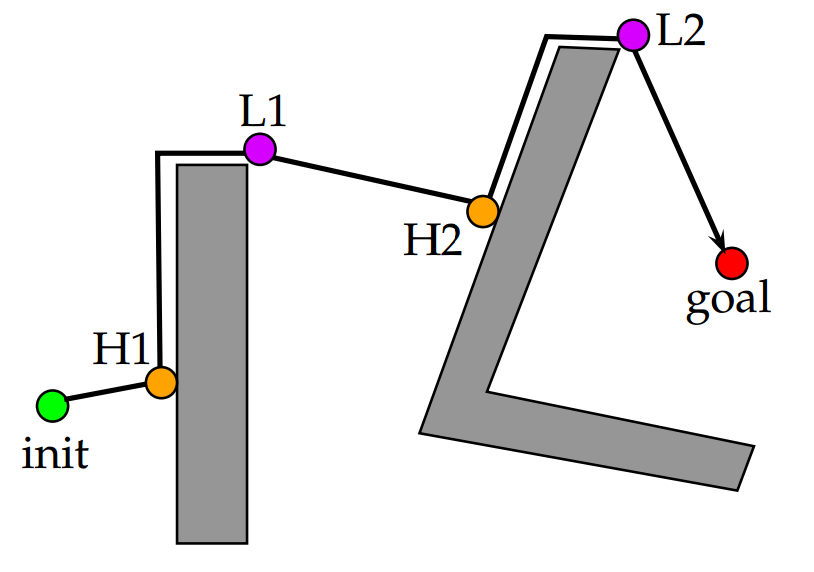
\includegraphics[width=0.7\linewidth]{figs/bug}

    \caption{This image shows an example of the bug algorithm determining hit
    points obstacles in order to move around them to reach the goal. This image
is courtesy of Dr.\ Erion Plaku.}

    \label{fig:bug}

\end{figure}

\section{Potential Fields}

\label{sec:costpf}

Using potential fields was an initial attempt to plan through uncertain dynamic
environments since they are frequently used to plan around dynamic obstacles
due to their reactive behaviour~\cite{pf, wallar_taros_2013,
wallar_ssci_2014_boids}.  The difference between the standard potential field
implementations and the one developed for this project was that the repulsive
obstacle field at a position $(x, y)$ was proportional to the cost distribution
at $(x, y)$ for a given time interval.  This is shown more formally in
Eq.~\ref{eq:badpotential}.

\begin{equation}
    U_{\Var{rep}}(p, t_0, t_m, A) = k \cdot P(p_x, p_y, t_0, t_m, A)
    \label{eq:badpotential}
\end{equation}

In Eq.~\ref{eq:badpotential}, the function $P$ is defined in Eq.~\ref{eq:prob},
and $k > 0$ is a constant.  The attractive potential field was kept the same as
the standard potential field implementation for robotic motion planning as
shown in Eq.~\ref{eq:badpotentialattr}

\begin{equation}
    U_{\Var{att}}(p, g) = c \cdot ||p - g||^2
    \label{eq:badpotentialattr}
\end{equation}

In Eq.~\ref{eq:badpotentialattr}, $c$ is a scaling constant such that $c > 0$.
The potential field planner would use the sum of these two fields to measure
the potential through the environment in order to eventually reach the goal by
successively moving to the area within the robot's sensing radius that had the
minimal potential.  Algo.~\ref{algo:pf} describes more formally how the
potential field planner generates a path through the environment.

\begin{algorithm}[ht]

    \caption{$\Function{PF}(q, g, O, A, R)$}

    \label{algo:pf}
    \begin{algorithmic}[1]
        \setcounter{ALC@line}{0}
        \vspace*{1mm}

        \STATE $q_{\Var{min}} \leftarrow q$
        \STATE $p_{\Var{min}} \leftarrow \infty$
        \STATE $\theta \leftarrow 0$
        \WHILE {$\theta \leq 2\pi$}
            \STATE $q' \leftarrow q + \delta t \cdot s \cdot
            \Function{Rot}(\theta)$
            \STATE $p \leftarrow U_{\Var{rep}}(q', O \cup A)
            + U_{\Var{att}}(q', g)$
            \IF {$p < p_{\Var{min}}$}
               \STATE $p_{\Var{min}} \leftarrow p$
                \STATE $q_{\Var{min}} \leftarrow q'$
            \ENDIF
            \STATE $\theta \leftarrow \theta + \delta \theta$
            \FORALL {$a \in A$}
                \STATE $\Function{Step}(a)$
            \ENDFOR
        \ENDWHILE

        \IF {$||q_{\Var{min}} - g|| < R$}
            \RETURN $\{p_{min}\}$
        \ENDIF

        \RETURN $\{q_{\Var{min}}\} \cup \Function{PF}(q_{\Var{min}}, g, O, A, R)$
    \end{algorithmic}
\end{algorithm}

Through some qualitative testing, these types of potential fields were still
leading the robot into unsafe areas and caused the robot to collide with the
dynamic obstacles regardless of velocity of the obstacles and the velocity of
the robot. After some manipulation of the constants used for the repulsive and
attractive potentials, there was only a nominal improvement which lead the
author to move towards sampling based motion planning techniques which are
outlined in Sec.~\ref{sec:stroadmap} and Sec.~\ref{sec:finaldesign}.

\section{Space-time Roadmap}

\label{sec:stroadmap}

The second attempt at devising a solution to the primary objective in
Ch.~\ref{chapter:objectives} was to create a three dimensional probabilistic
roadmap that can capture the connectivity of a two dimensional surface in
space-time. A spatio-temporal probabilistic roadmap (PRM) is a directed,
weighted graph, $(V, E)$, that represents the spatio-temporal connectivity of
the search space by randomly sampling points and connecting them such that if
$((i, t), (j, t')) \in E$, then both $i$ and $j$ must not collide with an
obstacle at times $t$ and $t'$ respectively, $||i - j|| \leq d$ where $d$
indicates the maximum distance away connected nodes can be from one another,
there must not be a collision with any obstacle along the edge from $i$ and $j$
in the time interval $[t, t']$, $|t - t'| < \delta t$, and $t < t'$~\cite{prm,
stprm}.  For the attempted space-time PRM, each node would be a vector, $(x, y,
t)$, which represents a two dimensional location, $(x, y)$, at a certain
absolute time $t$, and instead of randomly sampling a point in the environment,
a node in the graph would be randomly selected and propagated forward in time
by some random change in time such that the constraints for the roadmap are
still satisfied.  This algorithm is shown more formally in
Algo.~\ref{algo:diprm}.

\begin{algorithm}[ht]
    \caption{$\Function{TemporalRoadmap}(N, d, \delta t, s, p, O, A)$}
    \algorithmicrequire{
        \\$n$: Maximum number of samples
        \\$d$: Maximum distance between neighbouring nodes
        \\$O$: Set of obstacles
    }
    \\\algorithmicensure{
        \\An weighted directed graph of points describing where it is possible
        for the robot to move from its initial configuration.
    }
    \label{algo:diprm}
    \begin{algorithmic}[1]
        \setcounter{ALC@line}{0}
        \vspace*{1mm}

        \STATE $V \leftarrow \{(p, 0)\}$
        \FOR{$i = 1$ \TO $N$}
            \STATE $(n, t) \leftarrow \Function{RandomSelection}(V)$
            \STATE $t' \leftarrow t + \Function{UniformRandom}(\varepsilon, \delta t)$
            \STATE $\theta \leftarrow \Function{UniformRandom}(0, 2\pi)$
            \STATE $q \leftarrow n + s \cdot t' \cdot \Function{Rot}(\theta)$
            \IF{$\bigwedge_{o \in O} \neg \Function{Collision}(o, q)$}
                \FORALL {$(v, \tau) \in V$}
                    \IF {$||v - q|| < d \wedge |\tau - t'| < \delta t$}
                        \IF {$\tau < t'$}
                            \STATE $E \leftarrow E \cup \{((v, t), (v, t'),
                            C(v, q, \tau, t', A))\}$
                        \ELSE
                            \STATE $E \leftarrow E \cup \{((q, t'), (v, t),
                            C(q, v, t', \tau, A))\}$
                        \ENDIF
                    \ENDIF
                \ENDFOR
                \STATE $V \leftarrow V \cup \{(q, t)\}$
            \ENDIF
        \ENDFOR
        \RETURN $(V, E, W)$
    \end{algorithmic}
\end{algorithm}

With the generated roadmap, the first thought was to use a graph search
algorithm such as A*~\cite{astar} or Dijkstra's algorithm~\cite{dijkstra} to
find the path through the environment that had the lowest overall weight.  The
weight for an edge, $(i, j)$, defined as the line integral over the cost
surface for a given set of dynamic obstacles with a time interval of $[i_t,
j_t]$.  The notion of a cost distribution is described in
Ch.~\ref{chapter:methodology} and the formal equation for this line integral is
given in Eq.~\ref{eq:cost}.  This space-time roadmap approach yielded mixed
results.  The robot would sometimes evade the obstacles, but with the
incidence, the planner would lead the robot directly into a collision with a
dynamic obstacle. After some testing, it was discovered that since graph search
algorithms seek to find the path with minimum combined weight through the
graph, these algorithms are biased to return paths with a smaller number of
vertices.  This is because paths with a larger number of vertices will have a
higher overall weight. Since shortest path algorithms try to minimize this
overall weight, paths which may be safer but may take longer not be returned by
these algorithms.

To overcome this, instead of searching over the entire graph, the search could
be occur over the minimum spanning tree of the graph.  Since the roadmap is a
directed graph, Edmonds' algorithm~\cite{edmonds} was used since other minimum
spanning tree algorithms such as Kruskal's algorithm~\cite{kruskal} and Prim's
greedy algorithm~\cite{prim} only work on undirected graphs. Using the minimum
spanning tree would minimize the maximum cost associated with a path from the
initial configuration to the goal configuration thus moving the robot away from
high cost areas in space-time. Through qualitative analysis, this approach was
shown to still lead the robot to high cost areas and even into collisions with
obstacles.

This approach using a three dimensional probabilistic roadmap did not work in
practice regardless of the search algorithm because of the number of nodes that
need to be sampled in space-time in order for it to be effective.  The roadmap
indicates where in the environment the robot is able to travel to from a
starting location in space-time. If the number of nodes is too small the, the
goal may not even be in the graph, and thus the robot will never reach it.
Also, the less nodes in the graph the less optimal the generated path is, but
the more nodes added to the graph, the more computationally difficult it
becomes to search. Lastly, the main flaw with this approach is that biases the
sampling to areas that already have a high sample density and therefore may not
sample nodes in the goal area without having a high number of nodes in the
graph.

\section{Probabilistic Roadmap With Best First Search}

\label{sec:finaldesign}

After consideration for other sampling based motion planning techniques such as
rapidly exploring random trees~\cite{rrt} and expansive space trees~\cite{est}
the author chose to explore using a custom graph search algorithm over a two
dimensional probabilistic roadmap due to the lack of ability for classical
sampling based techniques to deal with time-dependent edge costs. The idea was
to use a probabilistic roadmap to capture the connectivity of the two
dimensional environment and to generate a search tree through the roadmap that
encodes the temporal information for each point in a tree node and is therefore
able to account for time-dependent edge costs. This graph search algorithm is a
temporal analogue of best-first search which tries to expand the best current
node in a search tree based on some heuristic~\cite{bestfs}. The heuristic in
this project is to expand the node in the search tree that has the minimum cost
as defined in Eq.~\ref{eq:cost}. A more complete and in depth description of
this method is given in Ch.~\ref{chapter:methodology}.

\end{document}
